\documentclass[a4paper,11pt]{article}
\usepackage{xeCJK}
\usepackage[margin=2cm]{geometry}
\usepackage{tikz}
\usetikzlibrary{positioning, arrows.meta}
\usepackage{amsmath,amssymb}

% 設定字體
\setCJKmainfont{Noto Sans TC}
\setmainfont{Noto Sans TC}

% 設定段落樣式
\setlength{\parskip}{0.5em}
\setlength{\parindent}{0em}

\begin{document}

\begin{center}
\Large \textbf{數學計算練習 - 詳解}
\end{center}

\noindent 生成日期:2025-04-29

\section*{第1回詳解}

% 問題 1 (帶圖)
\noindent\rule{\textwidth}{0.4pt}  % 分隔線
\begin{minipage}[t]{0.55\textwidth}
  \textbf{1.} 因為 $\cot \theta = \frac{1}{\tan \theta} = \frac{x}{y}$,即x座標除以y座標。
  
  當 $\theta = 60^\circ$ 時,點的座標為 $(\frac{1}{2}, \frac{\sqrt{3}}{2})$。
  
  所以 $\cot(60^\circ) = \frac{\frac{1}{2}}{\frac{\sqrt{3}}{2}} = \frac{1}{\sqrt{3}} = \frac{\sqrt{3}}{3}$。
\end{minipage}
\hfill
\begin{minipage}[t]{0.4\textwidth}
  \centering
  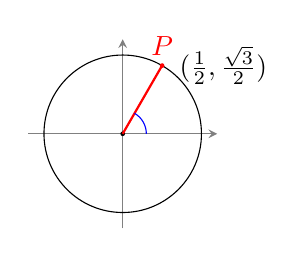
\begin{tikzpicture}[scale=1.0]
    % 坐標系
    \draw[-stealth, gray] (-1.2, 0) -- (1.2, 0);
    \draw[-stealth, gray] (0, -1.2) -- (0, 1.2);
    
    % 圓形
    \draw[thin, solid, black] (0.0, 0.0) circle (1.0);
    
    % 原點
    \fill[black] (0.0, 0.0) circle (0.03);
    
    % 點 P
    \fill[red] (0.5, 0.866) circle (0.03) node[above] {$P$};
    
    % 半徑
    \draw[thin, thick, red] (0.0, 0.0) -- (0.5, 0.866);
    
    % 角度
    \draw[thin, solid, blue] (0.0, 0.0) +(0.0:0.3) arc (0.0:60.0:0.3);
    
    % 標籤
    \node[right, black] at (0.6, 0.866) {$(\frac{1}{2},\frac{\sqrt{3}}{2})$};
  \end{tikzpicture}
  \vspace{0.5em}
  
  \centering \small{$\theta = 60^\circ$ 的單位圓}
\end{minipage}

% 問題 2 (帶圖)
\vspace{1em}
\noindent\rule{\textwidth}{0.4pt}  % 分隔線
\begin{minipage}[t]{0.55\textwidth}
  \textbf{2.} 因為 $\cot \theta = \frac{1}{\tan \theta} = \frac{x}{y}$,即x座標除以y座標。
  
  當 $\theta = 180^\circ$ 時,點的座標為 $(-1, 0)$。
  
  所以 $\cot(180^\circ) = \frac{-1}{0}$,這是未定義的,或者說是無窮大。
\end{minipage}
\hfill
\begin{minipage}[t]{0.4\textwidth}
  \centering
  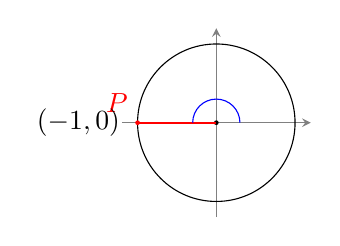
\begin{tikzpicture}[scale=1.0]
    % 坐標系
    \draw[-stealth, gray] (-1.2, 0) -- (1.2, 0);
    \draw[-stealth, gray] (0, -1.2) -- (0, 1.2);
    
    % 圓形
    \draw[thin, solid, black] (0.0, 0.0) circle (1.0);
    
    % 原點
    \fill[black] (0.0, 0.0) circle (0.03);
    
    % 點 P
    \fill[red] (-1.0, 0.0) circle (0.03) node[above left] {$P$};
    
    % 半徑
    \draw[thin, thick, red] (0.0, 0.0) -- (-1.0, 0.0);
    
    % 角度
    \draw[thin, solid, blue] (0.0, 0.0) +(0.0:0.3) arc (0.0:180.0:0.3);
    
    % 標籤
    \node[left, black] at (-1.1, 0.0) {$(-1,0)$};
  \end{tikzpicture}
  \vspace{0.5em}
  
  \centering \small{$\theta = 180^\circ$ 的單位圓}
\end{minipage}

% 問題 3 (帶圖)
\vspace{1em}
\noindent\rule{\textwidth}{0.4pt}  % 分隔線
\begin{minipage}[t]{0.55\textwidth}
  \textbf{3.} 因為 $\cos \theta = \frac{x}{r}$,即單位圓上點的x座標值。
  
  當 $\theta = 225^\circ$ 時,點的座標為 $(- \frac{\sqrt{2}}{2}, - \frac{\sqrt{2}}{2})$。
  
  所以 $\cos(225^\circ) = - \frac{\sqrt{2}}{2}$。
\end{minipage}
\hfill
\begin{minipage}[t]{0.4\textwidth}
  \centering
  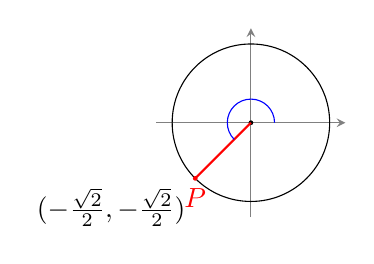
\begin{tikzpicture}[scale=1.0]
    % 坐標系
    \draw[-stealth, gray] (-1.2, 0) -- (1.2, 0);
    \draw[-stealth, gray] (0, -1.2) -- (0, 1.2);
    
    % 圓形
    \draw[thin, solid, black] (0.0, 0.0) circle (1.0);
    
    % 原點
    \fill[black] (0.0, 0.0) circle (0.03);
    
    % 點 P
    \fill[red] (-0.707, -0.707) circle (0.03) node[below] {$P$};
    
    % 半徑
    \draw[thin, thick, red] (0.0, 0.0) -- (-0.707, -0.707);
    
    % 角度
    \draw[thin, solid, blue] (0.0, 0.0) +(0.0:0.3) arc (0.0:225.0:0.3);
    
    % 標籤 - 調整位置避免超出邊界
    \node[below left, black] at (-0.707, -0.707) {$(- \frac{\sqrt{2}}{2},- \frac{\sqrt{2}}{2})$};
  \end{tikzpicture}
  \vspace{0.5em}
  
  \centering \small{$\theta = 225^\circ$ 的單位圓}
\end{minipage}

% 無圖問題 - 使用完整寬度
\vspace{1em}
\noindent\rule{\textwidth}{0.4pt}  % 分隔線
\noindent\textbf{4.} $\sin^{-1}(\frac{1}{2}) = 30^\circ$,因為 $\sin(30^\circ) = \sin(150^\circ) = \frac{1}{2}$ 但 $\sin^{-1}$ 的值域為 $[-90^\circ, 90^\circ]$,所以答案是 $30^\circ$。

\vspace{0.5em}
\noindent\rule{\textwidth}{0.4pt}  % 分隔線
\noindent\textbf{5.} $\sin^{-1}(\frac{1}{2}) = 30^\circ$,因為 $\sin(30^\circ) = \sin(150^\circ) = \frac{1}{2}$ 但 $\sin^{-1}$ 的值域為 $[-90^\circ, 90^\circ]$,所以答案是 $30^\circ$。

\vspace{0.5em}
\noindent\rule{\textwidth}{0.4pt}  % 分隔線
\noindent\textbf{6.} $\sqrt{2 \sqrt{154} + 29}$ \\
$= \sqrt{22+7 + 2\sqrt{22\cdot7}}$ \\
$= \sqrt{(\sqrt{22} + \sqrt{7})^2}$ \\
$= |\sqrt{22} + \sqrt{7}|$ \\
$= \sqrt{22} + \sqrt{7}$

\vspace{0.5em}
\noindent\rule{\textwidth}{0.4pt}  % 分隔線
\noindent\textbf{7.} $\sqrt{23 - 2 \sqrt{102}}$ \\
$= \sqrt{17+6 - 2\sqrt{17\cdot6}}$ \\
$= \sqrt{(\sqrt{17} - \sqrt{6})^2}$ \\
$= |\sqrt{17} - \sqrt{6}|$ \\
$= \sqrt{17} - \sqrt{6}$

\vspace{0.5em}
\noindent\rule{\textwidth}{0.4pt}  % 分隔線
\noindent\textbf{8.} $\sqrt{25 - 4 \sqrt{21}}$ \\
$= \sqrt{21+4 - 2\sqrt{21\cdot4}}$ \\
$= \sqrt{(\sqrt{21} - \sqrt{4})^2}$ \\
$= |\sqrt{21} - \sqrt{4}|$ \\
$= \sqrt{21} - 2$

\vspace{0.5em}
\noindent\rule{\textwidth}{0.4pt}  % 分隔線
\noindent\textbf{9.} $\sqrt{13 - 4 \sqrt{10}}$ \\
$= \sqrt{8+5 - 2\sqrt{8\cdot5}}$ \\
$= \sqrt{(\sqrt{8} - \sqrt{5})^2}$ \\
$= |\sqrt{8} - \sqrt{5}|$ \\
$= 2\sqrt{2} - \sqrt{5}$

\vfill
\begin{center}
\small{生成日期:2025-04-29}
\end{center}
\end{document}